\documentclass[a4paper,10pt,twocolumn,uplatex]{jsarticle}
\usepackage{style/nislab,style/resume}

%---------------------------------------------------------------------
% レジュメ種別・日付設定(要変更)
% \type{} 1:修士論文諮問会 2:卒業論文発表会 3:月例発表会 4:研究室合同発表会
%---------------------------------------------------------------------
\type{3}
\year{2022}
\month{2}
\date{4}

%---------------------------------------------------------------------
% ページ番号設定(要変更)
%---------------------------------------------------------------------
\setcounter{page}{7}

%---------------------------------------------------------------------
% 変更不要
%---------------------------------------------------------------------
\begin{document}

%---------------------------------------------------------------------
% タイトル作成部分(要変更)
% \maketitle{タイトル}{title}{名前}{name}
%---------------------------------------------------------------------
\maketitle{ホームネットワークにおけるデータ特性を考慮した\\SDNによる優先度制御手法}
{SDN Based Priority Control Method Considering Data Attributes for Home Network}
{国本 典晟}
{Tensei Kunimoto}

%---------------------------------------------------------------------
\section{はじめに}
Software-Defined Networking(SDN)技術の普及により,柔軟なネットワークの構築が可能となり,企業ネットワークやICTシステムに利用されている.一方,LAN環境を家庭内に構築したホームネットワークは,動画などの大容量データの増加やIoTデバイスの普及に伴い,通信帯域の逼迫が危惧されている.この問題の解決のため,SDN技術のホームネットワークへの適用が期待されている\cite{cisco}.
しかし,ホームネットワークには様々なアプリケーションによる特性の異なるデータが混在する.現在のインターネットサービスプロバイダ(ISP)はデータの特性を考慮せず同様に制御するため,通信帯域が逼迫した際に,重要なパケットの損失やQuality of Serviceの低下などの問題が生じる.
これに対して,データを遅延要件に基づき分類した研究\cite{framework}があるが,テレワークの増加など,昨今のリアルタイム性の高い通信の需要を十分に考慮できていない.
\par
本研究では,ホームネットワークのデータをリアルタイム性を含む特性を考慮して優先度を設定し分類する.その分類をもとに,通信帯域に合わせて優先度制御を行う手法を提案する.\par

%---------------------------------------------------------------------
\section{提案手法}
\subsection{概要}
提案手法の構成は図\ref{tab:proposal}に示すように,各家庭にはホームネットワークを家庭外のネットワークに接続するゲートウェイがあり,ゲートウェイはルータを介してISPのサーバと通信する.
SDNコントローラはホームネットワークの通信をリアルタイム性を含む特性から4つに分類し,それぞれの優先度制御に必要なメッセージをゲートウェイ,ルータ,ISPサーバとやり取りする.
また,制御において同じルールを持つ通信の集合であるフローのうち,優先度の高いフローの遅延やパケットロスを防ぐため,優先度の低いフローを意図的に破棄するアドミッション制御を行う.
SDNコントローラは通信帯域を監視し,必要に応じてアドミッション制御を行い,ゲートウェイにフローの破棄を指示する.\par

\begin{figure}[t]
	\begin{centering}
    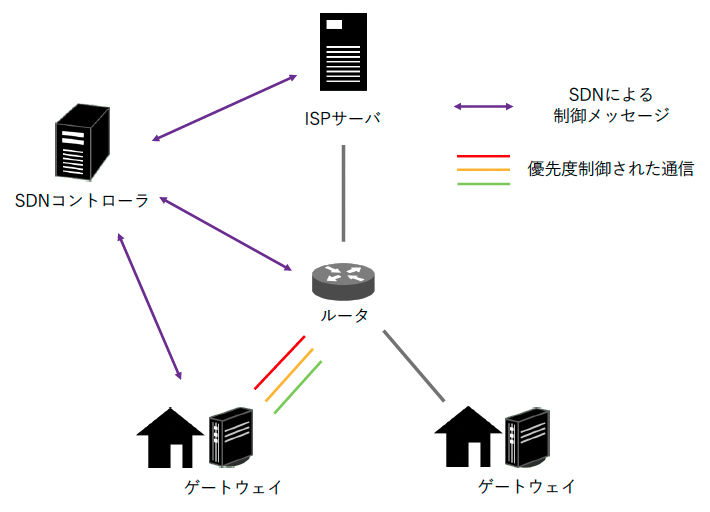
\includegraphics[width=\linewidth]{img/proposal.png}
    \caption{提案手法の構成}
    \label{tab:proposal}
    \end{centering}
\end{figure}

%---------------------------------------------------------------------
\subsection{優先度分類}
ホームネットワークの通信をリアルタイム性を含む特性を考慮して4つに分類し,優先度を設定する.
優先度1は侵入者センサや火災報知器などのミッションクリティカルなデータの通信である.遅延やパケットロスが許されず,通常あまり帯域を消費しないため,優先度は最も高い.
優先度2は音声通話やWeb会議など,リアルタイム性の高い音声・映像データの通信である.
優先度3は録画された動画など,リアルタイム性の低い音声・映像データの通信である.
優先度2の通信が途切れるとユーザ間の通話が途切れるなどの問題が生じるため,優先度3の通信よりも優先度を高く設定している.
優先度4はWebサイトなどのTCPによる通信や室温センサなどの非ミッションクリティカルなデータの通信である.遅延やパケットロスの影響が最も小さいため,最も低い優先度を設定する.\par

%---------------------------------------------------------------------
\subsection{アドミッション制御}
優先度1のフローはその特性から遅延やパケットロスをできる限り減らす必要があるため,アドミッション制御を行う.
アドミッション制御のフローチャートを図\ref{tab:adomission}に示す.
SDNコントローラが通信帯域を監視し,優先度1のフローの帯域が十分でない場合,優先度の低いフローから破棄することで,優先度1の帯域を確保するようにする.
しかし,ただ優先度の低いものから破棄するフローを選択した場合,同じフローが破棄され続け,通信が拒否される飢餓状態に陥る可能性がある.飢餓状態を回避するために,フロー毎に破棄された回数を記録する.破棄の候補となるフローが複数ある場合にそれぞれのフローが破棄された回数を参照し,少ない方を破棄の対象とすることで,飢餓状態を回避することができる.

\begin{figure}[t]
	\begin{centering}
    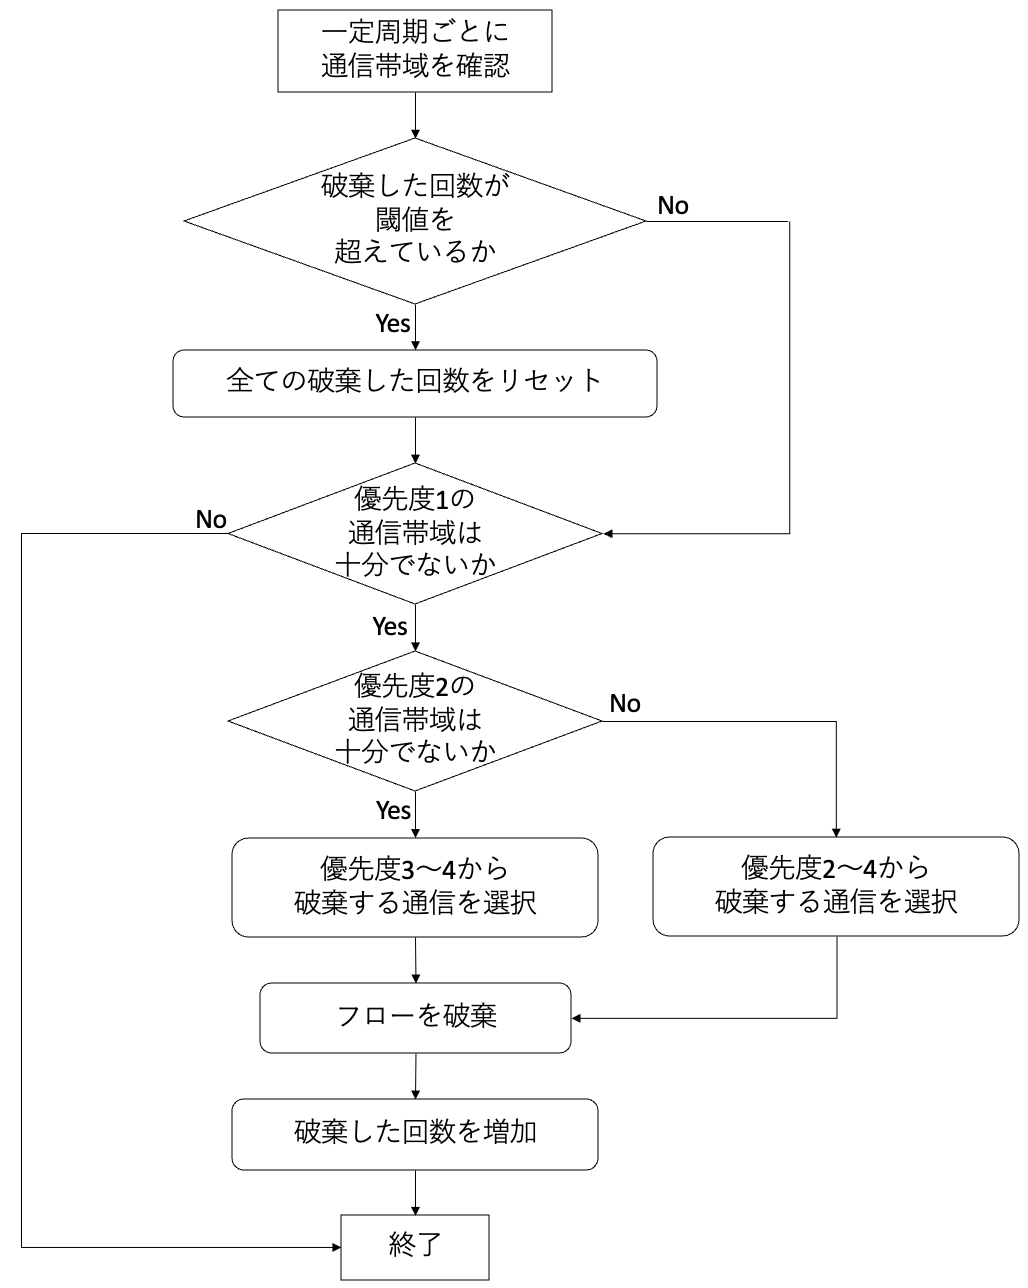
\includegraphics[width=0.75\linewidth]{img/adomission_test2.png}
    \caption{SDNコントローラにおけるアドミッション制御}
    \label{tab:adomission}
    \end{centering}
\end{figure}

%---------------------------------------------------------------------
\section{評価実験}
提案手法の動作手順を図\ref{tab:sequence}に示す.
SDNコントローラはOpenFlowプロトコルによりISPサーバ,ルータ,ゲートウェイと優先度制御に必要なメッセージをやり取りする.
ISPサーバはSDNコントローラに各フローの優先度を送信しておく.
ゲートウェイは\ref{priority}節で分類した4つの優先度の通信を行う.
ゲートウェイにはフローを保存するフローテーブルがある.
ゲートウェイはフローテーブルに適合するパケットを受信した場合はフロー通りに通信し,適合しないパケットを受信した場合はフローを確定させるために,適合しないパケットを受信したことを伝えるPacket\_InメッセージをSDNコントローラへ送信する.
SDNコントローラはゲートウェイからPacket\_Inメッセージを受信すると,優先度を分類し,ルータとゲートウェイにフローの情報を伝えるフローメッセージを送信する.
必要に応じてSDNコントローラはアドミッション制御を行い,ゲートウェイにフローの破棄を指示するフローメッセージを送信する.
実験は,提案手法の構成をネットワークエミュレータであるMininetを用いてネットワークを構築し,SDN構築フレームワークであるRyuを用いて行う.提案手法の有効性を検証するため,ネットワークパフォーマンスの測定ツールであるiperfを用いて,各優先度のパケットロス率,スループット,遅延を測定し,先行研究と比較する.
また,リアルタイム性の評価のため,優先度2と3のフローが破棄されたタイミングについて,先行研究と比較する.

\begin{figure}[t]
	\begin{centering}
    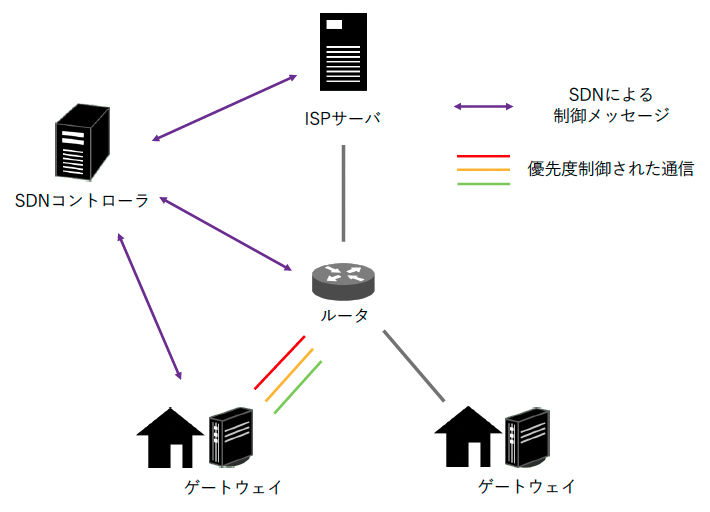
\includegraphics[width=\linewidth]{img/proposal.png}
    \caption{提案手法の動作手順}
    \label{tab:sequence}
    \end{centering}
\end{figure}

\section{まとめ}
本研究では,SDN技術のホームネットワークへの適用において,混在する異なる特性のデータの通信を制御するために,通信をリアルタイム性を含む特性から4つに分類し,優先度制御を行う手法を提案した.
提案手法について,ホームネットワークを想定して構築したネットワークにて実験を行い,先行研究と比較してリアルタイム性の点から有効性を示した.

%---------------------------------------------------------------------
% Bibliography(参考文献)
%---------------------------------------------------------------------
% thebibliography を利用する場合は以下を使用
\footnotesize{
  \begin{thebibliography}{99}
    \bibitem{cisco} Cisco Annual Internet Report(2018-2023)White Paper,https://www.cisco.com/c/en/us/solutions/collateral/executive-perspectives/annual-internet-report/white-paper-c11-741490.pdf(参照:2022/1).
    \bibitem{framework} Hung-Chin Jang, Chi-Wei Huang and Fu-Ku Yeh,Design A Bandwidth Allocation Framework for SDN Based Smart Home,\textit{2016 IEEE 7th Annual Information Technology, Electronics and Mobile Communication Conference (IEMCON)},pp.1-6,2016.
  \end{thebibliography}
}

% BibTex を利用する場合は以下を使用(初めての人には難しいかも)
% \bibliographystyle{junsrt}
% \bibliography{myref}

%---------------------------------------------------------------------
\end{document}
%---------------------------------------------------------------------
